% Asal-usul (tidak pernah dicetak): lihat sources/outline_sources.md (Tahun 1: insolasi menurut lintang dan musim, surplus dan defisit radiatif, transpor panas meridional oleh atmosfer dan samudra, panas laten). Soal dan nilai latihan dari kalkulator skrip Buku 3, calc/ch27.py; gambar dari figdata/bachelor-1/insolation.py (orbit Kepler di _solar.py) dan energy_balance.py (NCEP-NCAR Reanalysis 1, rerata jangka panjang 1991-2020, dataset bachelor-1-ncep-*).
% Fisika memiliki hukum kuadrat terbalik, benda hitam dan hukum Stefan-Boltzmann, musim dan panas laten (diingat kembali). Buku 2 (kelas 10) memberi seperempat konstanta matahari, diagram neraca global dan penutupannya, panas laten dan panas sensibel dengan kata-kata, kurva insolasi rata-rata tahunan, dan transpor ke arah kutub dengan kata-kata: di sini dibangun ulang dengan turunan dan data. Bab 1 memberi insolasi sesaat, deklinasi, serta terbit dan terbenamnya Matahari.
\chapter{Radiasi dan transpor panas}\label{ch:b1:radiation-heat-transport}

Dari sejuta mil jauhnya, permukaan Bumi yang terkena cahaya matahari tampak sebagai cakram laut biru, daratan cokelat, dan awan putih. Sinar matahari jatuh paling langsung di tengah cakram, dekat tropik, dan hanya menyerempet tepinya; tropik menyerap energi jauh lebih banyak daripada wilayah kutub. Namun tropik tidak makin panas dari tahun ke tahun, dan kutub tidak makin dingin. Angin dan arus samudra membawa kelebihan itu ke arah kutub, beberapa petawatt jumlahnya. Bab ini mengukur tiga suku neraca itu: sinar matahari yang diterima setiap \omterm{def:b1:spherical-astronomy:geographic}{lintang}, bagian yang diserap dan inframerah yang dikirim kembali ke angkasa, serta transpor yang mengisi selisihnya. Sebagian besar transpor berjalan dalam bentuk yang tak terlihat, sebagai uap air, yang panas lateninya dilepaskan di mana pun ia mengembun menjadi hujan.
% ledger: commons:epic-earth, trenberth:transport

\begin{omfigure}
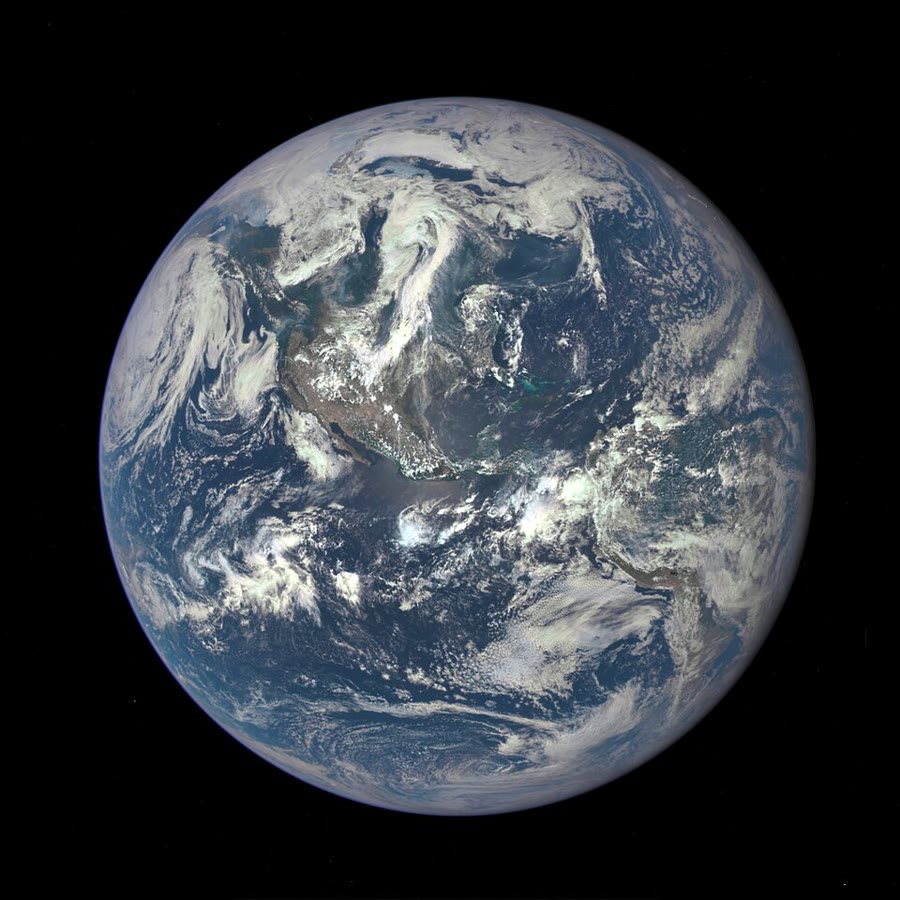
\includegraphics[width=0.55\linewidth]{images/book3/b1-epic-earth.jpg}

{\small Seluruh sisi Bumi yang terkena matahari, difoto pada 6 Juli 2015 oleh kamera di Deep Space Climate Observatory, sejuta mil jauhnya; Amerika Utara dan Tengah berada di tengah, dengan laut dangkal turkuois Karibia. Dua minggu setelah solstis Juni, Arktik di bagian atas diterangi sepanjang waktu. Awan yang cerah memantulkan banyak cahaya yang mencapainya; rona kebiruannya adalah sinar matahari yang dihamburkan oleh molekul udara. (NASA Goddard Space Flight Center, domain publik, melalui Wikimedia Commons.)}
\label{fig:b1:radiation-heat-transport:epic}
\end{omfigure}
% ledger: commons:epic-earth (polar day: figdata/bachelor-1/insolation.py)

\begin{recall}
\Cref{ch:b1:spherical-astronomy} mendefinisikan \omterm{def:b1:spherical-astronomy:insolation}{insolasi}, daya sinar matahari yang diterima per meter persegi permukaan horizontal di puncak atmosfer, $I = S_0(a/r)^2\sin h_\odot$ selama Matahari di atas, dengan $S_0 = \qty{1361}{W.m^{-2}}$ pada jarak rata-rata $a$; memberi ketinggian Matahari dari \omterm{def:b1:spherical-astronomy:equatorial}{sudut jamnya} $H$, deklinasinya $\delta$ dan \omterm{def:b1:spherical-astronomy:geographic}{lintang} $\varphi$, $\sin h_\odot = \sin\varphi\sin\delta + \cos\varphi\cos\delta\cos H$; dan \omterm{def:b1:spherical-astronomy:equatorial}{sudut jam} $H_0$ dari terbenamnya Matahari, $\cos H_0 = -\tan\varphi\tan\delta$ (\cref{prop:b1:spherical-astronomy:rising}). \Cref{ch:b1:comparative-planetology} mendefinisikan \omterm{def:b1:comparative-planetology:albedo}{albedo Bond} sebuah planet dan \omterm{def:b1:comparative-planetology:equilibrium-temperature}{suhu kesetimbangannya}. Buku-buku fisika memberikan hukum kuadrat terbalik untuk cahaya, radiasi benda hitam, $\sigma T^4$ per meter persegi dengan $\sigma = \qty{5.670e-8}{W.m^{-2}.K^{-4}}$ (Stefan--Boltzmann), dan panas laten perubahan keadaan. Buku~2 menunjukkan bahwa Bumi rata-rata menangkap seperempat konstanta matahari, menggambar neraca energi global Bumi dan memeriksa bahwa neraca itu seimbang, serta menjelaskan dengan kata-kata transpor panas ke arah kutub.
% ledger: earth:TSI, const:sigma, ipcc:budget-toa
\end{recall}

\section{Insolasi menurut lintang dan musim}\label{sec:b1:radiation-heat-transport:insolation}

\omterm{def:b1:spherical-astronomy:insolation}{Insolasi} sesaat berubah dari menit ke menit seiring Matahari melintasi langit. Untuk iklim, yang penting adalah jumlahnya selama sehari.

\begin{definition}[Insolasi harian rata-rata]\label{def:b1:radiation-heat-transport:daily-insolation}
\emph{Insolasi harian rata-rata}\index{insolasi harian rata-rata} $\bar Q$ pada suatu \omterm{def:b1:spherical-astronomy:geographic}{lintang} pada hari tertentu adalah \omterm{def:b1:spherical-astronomy:insolation}{insolasi} sesaat yang dirata-ratakan selama 24 jam hari itu, malam termasuk, dengan deklinasi Matahari dan jaraknya ditahan pada nilai harinya. Ia adalah daya per meter persegi permukaan horizontal di puncak atmosfer, dalam \unit{W.m^{-2}}.
\end{definition}

Menahan $\delta$ dan $r$ tetap untuk satu hari tidak berbahaya: deklinasi berubah paling banyak \ang{0.4} per hari, dan jarak kurang dari \qty{0.03}{\percent}.
% ledger: earth:obliquity, earth:ecc (computed in figdata/bachelor-1/insolation.py)

\begin{theorem}[Insolasi harian rata-rata]\label{thm:b1:radiation-heat-transport:daily}
Pada \omterm{def:b1:spherical-astronomy:geographic}{lintang} $\varphi$, pada hari ketika deklinasi Matahari adalah $\delta$ dan jaraknya $r$,
\[
  \bar Q = \frac{S_0}{\pi}\left(\frac{a}{r}\right)^{2}
  \bigl(h_0\sin\varphi\sin\delta + \cos\varphi\cos\delta\sin h_0\bigr),
\]
di mana $h_0 \in [0, \pi]$ adalah \omterm{def:b1:spherical-astronomy:equatorial}{sudut jam} terbenamnya Matahari dalam radian: $\cos h_0 =
-\tan\varphi\tan\delta$ bila $|\tan\varphi\tan\delta| \le 1$; $h_0 = \pi$ pada siang kutub ($\tan\varphi\tan\delta > 1$); $h_0 = 0$, dan $\bar Q = 0$, pada malam kutub ($\tan\varphi\tan\delta < -1$).
\end{theorem}

\begin{proof}
\omterm{def:b1:spherical-astronomy:equatorial}{Sudut jam} $H$ bertambah secara seragam melalui $2\pi$ dalam sehari, sehingga rerata atas hari sama dengan rerata atas $H \in [-\pi, \pi]$. Matahari berada di atas untuk $-h_0 < H < h_0$, tempat $\sin h_\odot > 0$, dan \omterm{def:b1:spherical-astronomy:insolation}{insolasinya} nol di luar itu. Karena itu
\[
  \bar Q = \frac{1}{2\pi}\int_{-h_0}^{h_0} S_0\left(\frac{a}{r}\right)^{2}
  \bigl(\sin\varphi\sin\delta + \cos\varphi\cos\delta\cos H\bigr)\,\mathrm dH ,
\]
yang sama dengan $(S_0/2\pi)(a/r)^2\bigl(2h_0\sin\varphi\sin\delta +
2\cos\varphi\cos\delta\sin h_0\bigr)$. Batasnya berasal dari \cref{prop:b1:spherical-astronomy:rising}: ketinggian nol bila $\cos H = -\tan\varphi\tan\delta$. Bila bilangan itu melebihi 1 dalam nilai mutlak, Matahari tidak pernah melintasi cakrawala: bila $\tan\varphi\tan\delta > 1$, integrannya positif untuk setiap $H$ dan integral berjalan sepanjang hari, $h_0 = \pi$; bila $\tan\varphi\tan\delta < -1$, ia negatif untuk setiap $H$ dan Matahari tidak pernah terbit.
\end{proof}

Dua kasus khusus perlu diingat di luar kepala. Di khatulistiwa, $\varphi = 0$ dan $h_0 = \pi/2$ apa pun musimnya:
\[
  \bar Q_\text{khatulistiwa} = \frac{S_0}{\pi}\left(\frac{a}{r}\right)^{2}\cos\delta ,
\]
terbesar pada ekuinoks, $S_0/\pi = \qty{433.2}{W.m^{-2}}$ pada jarak rata-rata.
Di kutub pada musim panasnya, $h_0 = \pi$ dan $\varphi = \pi/2$: $\bar Q_\text{kutub} =
S_0(a/r)^2\sin\delta$, Matahari berputar di langit pada ketinggian tetap yang sama dengan deklinasinya.
% ledger: earth:TSI

\begin{proposition}[Musim panas kutub]\label{prop:b1:radiation-heat-transport:polar-summer}
Pada hari dengan deklinasi $\delta > 0$, \omterm{def:b1:radiation-heat-transport:daily-insolation}{insolasi harian rata-rata} di Kutub Utara melebihi
yang di khatulistiwa jika dan hanya jika $\pi\tan\delta > 1$, yaitu $\delta >
\ang{17.66}$. Pada solstis Juni, $\delta = \ang{23.44}$, rasionya adalah $\pi\tan
\delta = 1.362$.
\end{proposition}

\begin{proof}
Dua kasus khusus di atas berbagi faktor $(S_0/\pi)(a/r)^2$; rasio keduanya adalah
$\pi\sin\delta/\cos\delta = \pi\tan\delta$, yang melebihi 1 bila $\tan\delta >
1/\pi$, $\delta > \arctan(1/\pi) = \ang{17.66}$. Dengan gradien sumbu,
$\pi\tan\ang{23.44} = 1.362$.
\end{proof}
% ledger: earth:obliquity

Dengan orbit Bumi, solstis Juni jatuh dekat aphelium, $(a/r)^2 = 0.968$: Kutub Utara
kemudian menerima \qty{524}{W.m^{-2}} sebagai rerata harian, khatulistiwa
\qty{385}{W.m^{-2}}. Enam bulan kemudian Kutub Selatan, dekat perihelium, menerima
\qty{559}{W.m^{-2}}, \qty{6.7}{\percent} lebih banyak daripada yang diterima Kutub Utara
pada musim panasnya: rasionya persis sama dengan rasio kedua nilai $(a/r)^2$. Gambar
di bawah menunjukkan $\bar Q$ sepanjang satu tahun. Maksimumnya berada di kutub pada
solstis; baji gelap adalah malam kutub, dibatasi oleh \omterm{def:b1:spherical-astronomy:geographic}{lintang} $\ang{90} -
|\delta|$;
titik subsolar, tempat Matahari melintas tepat di atas kepala pada tengah hari,
bergerak di antara tropik mengikuti deklinasi.
% ledger: earth:TSI, earth:ecc, earth:obliquity, nasa:earth-perihelion-longitude, usno:seasons-2026 (computed in figdata/bachelor-1/insolation.py)

\begin{omfigure}
\begin{tikzpicture}
\begin{axis}[omrecord, width=0.8\linewidth, height=6.4cm, view={0}{90},
  xmin=0, xmax=365, ymin=-90, ymax=90, xlabel={hari dalam tahun (dari 1 Januari)},
  ylabel={lintang (\unit{\degree})}, xtick={0,60,...,360}, ytick={-90,-60,...,90},
  colormap/viridis, colorbar, point meta min=0, point meta max=560,
  colorbar style={ylabel={$\bar Q$ (\unit{W.m^{-2}})}, ytick={0,100,...,500}, width=0.3cm},
  axis on top, grid=none]
% figdata/bachelor-1/insolation.py; ledger: earth:TSI, earth:ecc, earth:obliquity, nasa:earth-perihelion-longitude, usno:tropical-year, usno:seasons-2026
\addplot3[surf, shader=interp, mesh/ordering=y varies, mesh/rows=73]
  table[x=day, y=lat, z=Q] {figdata/out/bachelor-1-insolation-grid.dat};
\addplot3[white, dashed, line width=0.8pt] table[x=day, y=decl, z expr=600] {figdata/out/bachelor-1-insolation-sun.dat};
\addplot3[white, line width=0.6pt, unbounded coords=jump] table[x=day, y=night_n, z expr=600] {figdata/out/bachelor-1-insolation-sun.dat};
\addplot3[white, line width=0.6pt, unbounded coords=jump] table[x=day, y=night_s, z expr=600] {figdata/out/bachelor-1-insolation-sun.dat};
\node[font=\scriptsize, text=white] at (axis cs:28,81,700) {malam kutub};
\node[font=\scriptsize, text=white] at (axis cs:172,-81,700) {malam kutub};
\node[font=\scriptsize, text=white, anchor=south] at (axis cs:172,26,700) {lintang subsolar};
\end{axis}
\end{tikzpicture}

{\small \omterm{def:b1:radiation-heat-transport:daily-insolation}{Insolasi harian rata-rata} di puncak atmosfer terhadap hari dalam tahun dan \omterm{def:b1:spherical-astronomy:geographic}{lintang}, dari \cref{thm:b1:radiation-heat-transport:daily} dengan $S_0 = \qty{1361}{W.m^{-2}}$ dan orbit Bumi. Putus-putus: \omterm{def:b1:spherical-astronomy:geographic}{lintang} subsolar, sama dengan deklinasi; padat: tepi malam kutub. Kutub yang sedang musim panas menerima lebih banyak daripada tempat mana pun di Bumi; musim panas di selatan, dekat perihelium, adalah yang lebih terang dari keduanya.}
\label{fig:b1:radiation-heat-transport:matrix}
\end{omfigure}
% ledger: earth:TSI, earth:ecc, earth:obliquity, nasa:earth-perihelion-longitude, usno:seasons-2026

Dengan merata-ratakan $\bar Q$ sepanjang tahun diperoleh \omterm{def:b1:spherical-astronomy:insolation}{insolasi} rerata tahunan setiap \omterm{def:b1:spherical-astronomy:geographic}{lintang} (gambar di bawah): \qty{415.6}{W.m^{-2}} di khatulistiwa, \qty{328.3}{W.m^{-2}} pada \ang{40}, \qty{172.4}{W.m^{-2}} di kedua kutub. Musim panas kutub sangat terang tetapi musim dingin kutub gelap, dan sepanjang tahun khatulistiwa menerima \num{2.41} kali lebih banyak daripada kutub. Kurvanya sama di kedua belahan, meskipun musim panas di selatan lebih terang; \cref{exo:b1:radiation-heat-transport:10} menjelaskan mengapa.
% ledger: earth:TSI, earth:ecc, earth:obliquity (computed in figdata/bachelor-1/insolation.py)

\begin{omfigure}
\begin{tikzpicture}
\begin{axis}[omrecord, width=0.8\linewidth, height=5.6cm, xmin=-90, xmax=90, ymin=0, ymax=600,
  xlabel={lintang (\unit{\degree})}, ylabel={$\bar Q$ (\unit{W.m^{-2}})},
  xtick={-90,-60,...,90}, ytick={0,100,...,600}]
% figdata/bachelor-1/insolation.py; ledger: earth:TSI, earth:ecc, earth:obliquity, nasa:earth-perihelion-longitude
\addplot[omThm, line width=0.8pt] table[x=lat, y=Q_jun] {figdata/out/bachelor-1-insolation-annual.dat};
\addplot[omDef, line width=0.8pt] table[x=lat, y=Q_dec] {figdata/out/bachelor-1-insolation-annual.dat};
\addplot[black, line width=1.1pt] table[x=lat, y=Q_ann] {figdata/out/bachelor-1-insolation-annual.dat};
\addplot[black!60, dashed, domain=-90:90] {340.30};
\node[font=\scriptsize, text=omThm, anchor=west] at (axis cs:50,540) {solstis Juni};
\node[font=\scriptsize, text=omDef, anchor=east] at (axis cs:-50,575) {solstis Desember};
\node[font=\scriptsize, anchor=north] at (axis cs:-72,160) {rerata tahunan};
\node[font=\scriptsize, text=black!60, anchor=south west] at (axis cs:-88,342) {rerata global};
\end{axis}
\end{tikzpicture}

{\small \omterm{def:b1:radiation-heat-transport:daily-insolation}{Insolasi harian rata-rata} terhadap \omterm{def:b1:spherical-astronomy:geographic}{lintang} pada kedua solstis, dan rerata tahunannya (hitam). Rerata tahunan melebihi rerata global, \qty{340.3}{W.m^{-2}} (putus-putus), antara \ang{37} LS dan \ang{37} LU, pada \qty{60}{\percent} permukaan Bumi.}
\label{fig:b1:radiation-heat-transport:annual}
\end{omfigure}
% ledger: earth:TSI, earth:ecc, earth:obliquity (computed in figdata/bachelor-1/insolation.py)

\begin{proposition}[Rerata global]\label{prop:b1:radiation-heat-transport:global}
Pada setiap saat, \omterm{def:b1:spherical-astronomy:insolation}{insolasi} yang dirata-ratakan atas seluruh bola adalah $\tfrac14
S_0(a/r)^2$. Dirata-ratakan juga atas setahun, ia adalah $S_0/(4\sqrt{1 - e^2})$, dengan
$e$ eksentrisitas orbit: \qty{340.30}{W.m^{-2}} untuk Bumi, dalam
\qty{0.02}{\percent} dari $S_0/4 = \qty{340.25}{W.m^{-2}}$.
\end{proposition}

\begin{proof}
Bumi, berjari-jari $R$, menangkap sinar matahari yang melintasi cakram seluas $\pi
R^2$, daya $S_0(a/r)^2\pi R^2$, yang jatuh pada belahan siang; disebarkan ke seluruh
permukaan $4\pi R^2$, ia memberi hasil pertama. Rerata waktu dari
$(a/r)^2$ atas orbit adalah $1/\sqrt{1-e^2}$
(\cref{exo:b1:radiation-heat-transport:11}).
\end{proof}
% ledger: earth:TSI, earth:ecc

\section{Radiasi yang diserap dan dipancarkan}\label{sec:b1:radiation-heat-transport:toa}

Dari sinar matahari yang diterima suatu \omterm{def:b1:spherical-astronomy:geographic}{lintang}, ia memantulkan sebagian langsung kembali, dari awan, salju, es, gurun dan, dalam derajat yang lebih kecil, laut; sisanya diserapnya, di udara dan di permukaan. Ia juga kehilangan energi dengan memancarkan radiasi inframerah ke angkasa, siang dan malam.

\begin{definition}[Radiasi gelombang panjang keluar]\label{def:b1:radiation-heat-transport:olr}
\emph{Radiasi gelombang panjang keluar}\index{radiasi gelombang panjang keluar} (OLR)
adalah daya radiasi inframerah yang meninggalkan puncak atmosfer menuju angkasa, per
meter persegi. \emph{Suhu emisi}\index{suhu emisi} $T_e$ adalah suhu benda hitam yang
memancarkan daya yang sama: $\sigma T_e^4 = \text{OLR}$.
\end{definition}

OLR sebagian berasal dari permukaan, melalui udara yang transparan bagi inframerah, dan
sebagian dari udara serta puncak awan yang lebih tinggi. \omterm{def:b1:radiation-heat-transport:olr}{Suhu emisi} adalah sifat
radiasinya, bukan suhu suatu aras tertentu: ia lebih rendah daripada suhu tanah di
bawahnya, karena lapisan yang memancarkan lebih dingin.
% ledger: ipcc:budget-surface, ipcc:budget-toa

\begin{definition}[Radiasi bersih; surplus dan defisit radiatif]\label{def:b1:radiation-heat-transport:net-radiation}
\emph{Radiasi bersih}\index{radiasi bersih} di puncak atmosfer adalah
\[
  R = \underbrace{(1 - \alpha)\,\bar Q}_{\text{matahari terserap}} - \text{OLR},
\]
di mana $\alpha$ adalah albedo lokal, bagian sinar matahari datang yang dipantulkan ke angkasa; ketiga besaran itu adalah rerata tahunan pada satu \omterm{def:b1:spherical-astronomy:geographic}{lintang}. \omterm{def:b1:spherical-astronomy:geographic}{Lintang} dengan $R > 0$ memiliki \emph{surplus radiatif}\index{surplus radiatif}; yang dengan $R < 0$ memiliki \emph{defisit radiatif}\index{defisit radiatif}.
\end{definition}

Untuk seluruh Bumi, \omterm{def:b1:radiation-heat-transport:net-radiation}{radiasi bersih} rata-rata harus hampir nol, karena planet ini tidak memanas atau mendingin lebih dari beberapa persepuluh watt per meter persegi: penilaian terakhir menempatkan ketidakseimbangan pada \qty{0.7}{W.m^{-2}}, dari \qty{340}{W.m^{-2}} masuk, yang \qty{100}{W.m^{-2}} dipantulkan (albedo global
\num{0.294}) dan \qty{239}{W.m^{-2}} keluar sebagai inframerah.
% ledger: ipcc:budget-toa, earth:albedo

Profil zonal bab ini berasal dari reanalisis, yaitu sistem prakiraan cuaca yang dijalankan selama beberapa dekade terakhir, yang mengasimilasi observasi setiap hari dan menghasilkan keadaan atmosfer yang lengkap dan konsisten. Reanalisis yang dipakai di sini, sejak 1948, memberi rerata bulanan pada kisi 94 \omterm{def:b1:spherical-astronomy:geographic}{lintang} dan 192 \omterm{def:b1:spherical-astronomy:geographic}{bujur}; bab ini memakai rerata 1991--2020-nya. Fluks radiasinya adalah keluaran model, yaitu prakiraan yang dibatasi oleh observasi. Gambar di bawah menunjukkan rerata zonalnya terhadap $\sin\varphi$, sehingga selang yang sama pada sumbu berarti luas yang sama pada bola.
% ledger: psl:ncep-r1, kalnay96:reanalysis, data:b3-ncep

\begin{omfigure}
\begin{tikzpicture}
\begin{axis}[omrecord, width=0.8\linewidth, height=6cm, xmin=-1, xmax=1, ymin=0, ymax=320,
  xlabel={lintang (\unit{\degree}, sumbu dalam $\sin\varphi$)}, ylabel={fluks (\unit{W.m^{-2}})},
  xtick={-0.866,-0.5,0,0.5,0.866}, xticklabels={60 LS,30 LS,0,30 LU,60 LU},
  ytick={0,50,...,300}]
% figdata/bachelor-1/energy_balance.py; ledger: data:b3-ncep, psl:ncep-r1
\addplot[name path=asr, omProp, line width=1pt] table[x expr={sin(\thisrow{lat})}, y=asr] {figdata/out/bachelor-1-energy_balance-toa.dat};
\addplot[name path=olr, omThm, line width=1pt] table[x expr={sin(\thisrow{lat})}, y=olr] {figdata/out/bachelor-1-energy_balance-toa.dat};
\addplot[omProp!25] fill between[of=asr and olr, split, every segment no 1/.style={omDef!18}, every segment no 2/.style={omProp!30}, every segment no 3/.style={omDef!18}];
\node[font=\scriptsize, text=omProp!80!black] at (axis cs:-0.55,300) {matahari terserap};
\node[font=\scriptsize, text=omThm] at (axis cs:-0.2,226) {OLR};
\node[font=\scriptsize] at (axis cs:0,262) {surplus};
\node[font=\scriptsize] at (axis cs:0.86,178) {defisit};
\node[font=\scriptsize] at (axis cs:-0.86,178) {defisit};
\end{axis}
\end{tikzpicture}

{\small Rerata zonal dan tahunan radiasi matahari yang terserap (oranye) dan \omterm{def:b1:radiation-heat-transport:olr}{radiasi gelombang panjang keluar} (merah) di puncak atmosfer, dari Reanalysis~1 NCEP-NCAR, rerata 1991--2020 (data disediakan oleh NOAA PSL, Boulder, Colorado, AS, dari situs webnya di https://psl.noaa.gov). Diarsir: \omterm{def:b1:radiation-heat-transport:net-radiation}{surplus radiatif} \omterm{def:b1:spherical-astronomy:geographic}{lintang} rendah dan defisit \omterm{def:b1:spherical-astronomy:geographic}{lintang} tinggi.}
\label{fig:b1:radiation-heat-transport:toa}
\end{omfigure}
% ledger: data:b3-ncep, psl:ncep-r1, kalnay96:reanalysis

Kedua kurva memiliki bentuk yang sangat berbeda. Sinar matahari yang terserap turun dari \qty{288}{W.m^{-2}} di dekat khatulistiwa menjadi \qty{76}{W.m^{-2}} pada \ang{81} LU, dengan faktor \num{3.8}: \omterm{def:b1:spherical-astronomy:insolation}{insolasi} turun, dan albedo naik dari \num{0.31} menjadi \num{0.57}, bersama Matahari yang rendah, salju dan es laut. OLR hanya turun dari \qty{245}{W.m^{-2}} menjadi \qty{192}{W.m^{-2}}, dengan faktor \num{1.27}; \omterm{def:b1:radiation-heat-transport:olr}{suhu emisinya} \qty{256}{K} dan \qty{241}{K}. OLR bahkan sedikit lebih rendah di khatulistiwa, \qty{245}{W.m^{-2}}, daripada dekat \ang{20}, \qty{269}{W.m^{-2}}: awan sabuk hujan khatulistiwa menjulang tinggi dan puncaknya yang dingin memancarkan sedikit, sedangkan langit subtropis yang lebih cerah membiarkan lebih banyak inframerah lolos. Di mana pun sinar matahari yang terserap melebihi OLR, \omterm{def:b1:spherical-astronomy:geographic}{lintang} itu memiliki surplus.
% ledger: data:b3-ncep (values computed in figdata/bachelor-1/energy_balance.py)

\begin{example}[Anggaran global reanalisis]\label{ex:b1:radiation-heat-transport:global}
Dirata-ratakan atas globe, reanalisis ternyata menerima \qty{341.9}{W.m^{-2}}, memantulkan \qty{117.0}{W.m^{-2}} (albedo \num{0.342}), menyerap \qty{224.8}{W.m^{-2}} dan memancarkan \qty{237.7}{W.m^{-2}}: \omterm{def:b1:radiation-heat-transport:net-radiation}{radiasi bersih} \qty{-12.9}{W.m^{-2}}. OLR berada dalam \qty{1.3}{W.m^{-2}} dari \qty{239}{W.m^{-2}} yang dinilai, tetapi pantulannya \qty{17}{W.m^{-2}} lebih besar daripada \qty{100}{W.m^{-2}} yang dinilai. Ketidakseimbangan nyata sebesar ini akan mendinginkan Bumi sebesar \qty{6.6}{PW}; itu adalah galat model, bukan sifat Bumi, dan transpor di bawah dihitung setelah rerata global dihilangkan.
% ledger: data:b3-ncep, ipcc:budget-toa (computed in figdata/bachelor-1/energy_balance.py)
\end{example}

\section{Transpor panas meridional}\label{sec:b1:radiation-heat-transport:transport}

\begin{definition}[Transpor panas meridional]\label{def:b1:radiation-heat-transport:mht}
\emph{Transpor panas meridional}\index{transpor panas meridional} $T(\varphi)$
melintasi sejajar \omterm{def:b1:spherical-astronomy:geographic}{lintang} $\varphi$ adalah energi yang dibawa ke utara melintasi sejajar
itu per satuan waktu, oleh atmosfer dan samudra bersama, dalam rerata tahunan. Ia dihitung
positif ke utara dan diukur dalam petawatt (\qty{1}{PW} = \qty{e15}{W}).
\end{definition}

\begin{proposition}[Transpor dari radiasi bersih]\label{prop:b1:radiation-heat-transport:mht}
Jika energi yang tersimpan di setiap pita \omterm{def:b1:spherical-astronomy:geographic}{lintang} tidak berubah dari tahun ke tahun, maka untuk Bumi berjari-jari $a_\oplus$,
\[
  T(\varphi) = 2\pi a_\oplus^2\int_{-\pi/2}^{\varphi} R(\varphi')\cos\varphi'\,
  \mathrm d\varphi' = -2\pi a_\oplus^2\int_{\varphi}^{\pi/2} R(\varphi')\cos
  \varphi'\,\mathrm d\varphi' ,
\]
dan $T$ mencapai ekstrem pada \omterm{def:b1:spherical-astronomy:geographic}{lintang} tempat $R$ berubah tanda.
\end{proposition}

\begin{proof}
Ambil tudung kutub di selatan sejajar $\varphi$ sebagai volume kontrol, dari dasar
samudra hingga puncak atmosfer (gambar di bawah). Energi masuk atau keluar hanya lewat dua cara:
sebagai radiasi di puncak, daya bersih
$\int R\,\mathrm dA$, dan melalui transpor di tepinya, $-T(\varphi)$ (transpor ke utara
meninggalkan tudung selatan). Pita antara $\varphi'$ dan
$\varphi' + \mathrm d\varphi'$ memiliki luas $\mathrm dA = 2\pi a_\oplus\cos\varphi'
\cdot a_\oplus\,\mathrm d\varphi'$. Tanpa perubahan penyimpanan, jumlahnya nol:
$\int_{-\pi/2}^{\varphi} R\,2\pi a_\oplus^2\cos\varphi'\,\mathrm d\varphi' -
T(\varphi) = 0$. Diterapkan pada seluruh Bumi ($\varphi = \pi/2$, tanpa tepi), keseimbangan yang sama
memberi $\int R\,\mathrm dA = 0$ atas bola, dari situ bentuk kedua.
Dengan diferensiasi, $T'(\varphi) = 2\pi a_\oplus^2 R(\varphi)\cos\varphi$, yang
lenyap di tempat $R$ berubah tanda.
\end{proof}
% ledger: earth:Rmean

\begin{omfigure}
\begin{tikzpicture}[>={Stealth[length=2mm]}, font=\scriptsize]
  \def\R{2.0}
  \def\ph{40}
  \fill[omDef!12] ({-\R*cos(\ph)},{\R*sin(\ph)}) arc[start angle=180-\ph, end angle=\ph, radius=\R]
     -- ({\R*cos(\ph)},{\R*sin(\ph)}) arc[start angle=0, end angle=-180, x radius={\R*cos(\ph)}, y radius={0.25*\R*cos(\ph)}] -- cycle;
  \draw[thick] (0,0) circle (\R);
  \draw[black!40] (-\R,0) arc[start angle=180, end angle=360, x radius=\R, y radius={0.25*\R}];
  \draw[black!40, dashed] (\R,0) arc[start angle=0, end angle=180, x radius=\R, y radius={0.25*\R}];
  \draw[omDef, thick] ({-\R*cos(\ph)},{\R*sin(\ph)}) arc[start angle=180, end angle=360, x radius={\R*cos(\ph)}, y radius={0.25*\R*cos(\ph)}];
  \draw[omDef, thick, dashed] ({\R*cos(\ph)},{\R*sin(\ph)}) arc[start angle=0, end angle=180, x radius={\R*cos(\ph)}, y radius={0.25*\R*cos(\ph)}];
  \node[anchor=west, black!60] at (\R+0.05,0) {khatulistiwa};
  \node[anchor=west, omDef] at ({\R*cos(\ph)+0.1},{\R*sin(\ph)}) {sejajar $\varphi$};
  \foreach \x in {-0.55,0.55} \draw[->, very thick, omProp] (\x,{\R*sin(\ph)-0.75}) -- (\x,{\R*sin(\ph)-0.1});
  \node[omProp!80!black, anchor=east] at ({-\R-0.1},{\R*sin(\ph)-0.4}) {$T(\varphi)$ melintasi tepi};
  \foreach \a in {65,90,115} {
    \draw[->, omThm, decorate, decoration={snake, amplitude=0.6mm, segment length=2mm, post length=1.5mm}]
      ({(\R+0.05)*cos(\a)},{(\R+0.05)*sin(\a)}) -- ({(\R+0.75)*cos(\a)},{(\R+0.75)*sin(\a)});
  }
  \node[omThm, anchor=south] at (0,\R+0.8) {radiasi bersih $R < 0$ di atas tudung};
\end{tikzpicture}

{\small Volume kontrol \cref{prop:b1:radiation-heat-transport:mht}, digambar untuk tudung di utara sejajar $\varphi$ (diarsir): dalam keadaan tunak, apa yang hilang dari tudung melalui radiasi di puncak atmosfer (merah) adalah apa yang dibawa masuk oleh atmosfer dan samudra melintasi tepinya (oranye).}
\label{fig:b1:radiation-heat-transport:cap}
\end{omfigure}

Diterapkan pada reanalisis, dengan rerata global \qty{-12.9}{W.m^{-2}} dikurangkan dari $R$ di setiap \omterm{def:b1:spherical-astronomy:geographic}{lintang}, proposisi memberi kurva di bawah. Transpor mengarah ke utara di belahan utara dan ke selatan di belahan selatan, selalu menuju kutub. Ia mencapai puncak \qty{4.1}{PW} dekat \ang{38} LU dan \qty{4.5}{PW} dekat \ang{32} LS, tempat $R$ dikurangi rerataannya berubah tanda; di \ang{40} LU ia adalah \qty{4.11}{PW}. Ia kecil di khatulistiwa, tempat surplus setiap belahan diekspor ke kutubnya sendiri.
% ledger: data:b3-ncep (computed in figdata/bachelor-1/energy_balance.py)

\begin{omfigure}
\begin{tikzpicture}
\begin{axis}[omrecord, width=0.8\linewidth, height=6cm, xmin=-90, xmax=90, ymin=-5.5, ymax=6.4,
  xlabel={lintang (\unit{\degree})}, ylabel={transpor ke utara (\unit{PW})},
  xtick={-90,-60,...,90}, ytick={-4,-2,...,4}]
% figdata/bachelor-1/energy_balance.py; ledger: data:b3-ncep, trenberth:transport
\addplot[black!40, domain=-90:90] {0};
\addplot[black, line width=1.1pt] table[x=lat, y=T_PW] {figdata/out/bachelor-1-energy_balance-transport.dat};
\addplot[omMeth, dashed, line width=0.9pt] table[x=lat, y=T_PW] {figdata/out/bachelor-1-energy_balance-latent.dat};
\addplot[only marks, mark=square*, mark size=2pt, omThm] coordinates {(43,5.0)};
\node[font=\scriptsize, anchor=east] at (axis cs:28,4.4) {total};
\node[font=\scriptsize, text=omMeth, anchor=north] at (axis cs:42,0.9) {panas laten};
\node[font=\scriptsize, text=omThm, anchor=south] at (axis cs:43,5.2) {atmosfer saja (Trenberth dan Caron)};
\end{axis}
\end{tikzpicture}

{\small \omterm{def:b1:radiation-heat-transport:mht}{Transpor panas meridional} yang diimplikasikan oleh \omterm{def:b1:radiation-heat-transport:net-radiation}{radiasi bersih} reanalisis (hitam) dan bagian panas latennya (hijau putus-putus, dari penguapan dan presipitasi, \cref{sec:b1:radiation-heat-transport:latent}); NCEP-NCAR Reanalysis~1, rerata 1991--2020, data disediakan oleh NOAA PSL. Persegi: puncak transpor atmosfer saja dalam perkiraan yang dibatasi oleh pengukuran radiasi dari satelit, \qty{5.0}{PW} pada \ang{43} LU (Trenberth dan Caron, 2001).}
\label{fig:b1:radiation-heat-transport:transport}
\end{omfigure}
% ledger: data:b3-ncep, psl:ncep-r1, trenberth:transport

Persegi pada gambar adalah peringatan. Sebuah studi atas tahun 1985--1989, ketika sebuah eksperimen satelit mengukur radiasi di puncak atmosfer dengan andal, menghitung transpor atmosfer dari angin, suhu dan kelembapan dari dua reanalisis: atmosfer saja membawa \qty{5.0}{PW} pada \ang{43} LU, lebih dari \qty{4.0}{PW} reanalisis ini untuk atmosfer dan samudra bersama. Studi yang sama menemukan bahwa fluks yang dihasilkan model reanalisis kurang sesuai dengan perkiraan samudra yang independen daripada fluks yang diturunkan dari observasi. Setelah rerata global dihilangkan, transpor hanya bergantung pada bagaimana $R$ bervariasi terhadap \omterm{def:b1:spherical-astronomy:geographic}{lintang}, dan \omterm{def:b1:radiation-heat-transport:net-radiation}{radiasi bersih} reanalisis ini bervariasi terlalu sedikit dari tropik ke kutub. Bentuk kurvanya, puncaknya di \omterm{def:b1:spherical-astronomy:geographic}{lintang} menengah dan kesimetrisannya yang hampir sempurna, dapat dipercaya; tingginya setidaknya kurang seperlima.
% ledger: trenberth:transport, tc01:method, data:b3-ncep (computed in figdata/bachelor-1/energy_balance.py)

Siapa yang membawa panas? Studi yang sama menemukan bahwa samudra membawa lebih banyak daripada atmosfer hanya antara khatulistiwa dan \ang{17} LU; pada \ang{35}, tempat transpor total mencapai puncaknya di setiap belahan, atmosfer membawa \qty{78}{\percent} darinya di utara dan \qty{92}{\percent} di selatan. Bagian samudra dibahas dalam \cref{ch:b1:ocean-circulation}, bagian atmosfer dalam \cref{ch:b1:atmospheric-circulation}.
% ledger: trenberth:transport

\begin{method}[Transpor dari pita zonal]\label{met:b1:radiation-heat-transport:bands}
\begin{enumerate}
  \item Bagi tudung di sebelah kutub dari \omterm{def:b1:spherical-astronomy:geographic}{lintang} yang diminati menjadi pita-pita; untuk setiap pita, ambil rerata \omterm{def:b1:spherical-astronomy:insolation}{insolasi} $\bar Q_i$, albedo $\alpha_i$ dan OLR$_i$.
  \item Hitung \omterm{def:b1:radiation-heat-transport:net-radiation}{radiasi bersih} setiap pita, $R_i = (1 - \alpha_i)\bar Q_i -
        \text{OLR}_i$, dan kurangkan rerata global $R$ bila tidak nol.
  \item Hitung luas setiap pita, $A_i = 2\pi a_\oplus^2(\sin\varphi_{i,2} -
        \sin\varphi_{i,1})$, dengan $a_\oplus = \qty{6371}{km}$.
  \item Transpor melintasi tepi adalah minus daya bersih tudung, $-\sum_i R_i A_i$, positif ke arah kutub; bagi dengan \num{e15} untuk petawatt.
\end{enumerate}
\end{method}
% ledger: earth:Rmean

\section{Panas laten dan sensibel}\label{sec:b1:radiation-heat-transport:latent}

Permukaan Bumi menyerap sebagian besar sinar matahari, tetapi atmosfer memancarkan sebagian besar inframerah ke angkasa. Permukaan menyerahkan energi kepada udara dengan tiga cara: melalui radiasi inframerahnya sendiri, dengan memanaskan udara yang bersentuhan dengannya, dan dengan menguapkan air, yang panas lateninya dilepaskan di mana pun uap itu mengembun. Tempat itu bisa berjarak ribuan kilometer: panas laten berjalan bersama angin.

\begin{definition}[Fluks panas laten dan sensibel; rasio Bowen]\label{def:b1:radiation-heat-transport:surface-fluxes}
\emph{Fluks panas laten}\index{fluks panas laten} $LE$ adalah daya per meter persegi yang hilang dari permukaan karena penguapan: laju penguapan $E$, dalam
\unit{kg.m^{-2}.s^{-1}}, dikali panas laten penguapan $L$. \emph{Fluks panas sensibel}\index{fluks panas sensibel} $H$ adalah daya per meter persegi yang diteruskan permukaan ke udara secara konduksi dan turbulensi, sehingga memanaskannya. Keduanya dihitung positif ke atas. Rasionya $B = H/LE$ adalah \emph{rasio Bowen}\index{rasio Bowen}.
\end{definition}

Pada sekitar \qty{15}{\celsius}, $L = \qty{2.4655}{MJ.kg^{-1}}$. \omterm{def:b1:radiation-heat-transport:surface-fluxes}{Rasio Bowen} kecil
di atas laut dan di atas tanah basah, tempat air melimpah, dan besar di atas daratan kering.
Dalam reanalisis ia adalah \num{0.09} di khatulistiwa, \num{0.37} pada \ang{25} LU,
\omterm{def:b1:spherical-astronomy:geographic}{lintang} gurun panas yang besar, dan negatif pada \ang{70} LU, tempat permukaan salju
dan es lebih dingin daripada udara di atasnya dalam rerata tahunan, sehingga panas
sensibel mengalir ke bawah. Dirata-ratakan atas globe, reanalisis memberi $LE =
\qty{82.5}{W.m^{-2}}$ dan $H = \qty{15.2}{W.m^{-2}}$, \omterm{def:b1:radiation-heat-transport:surface-fluxes}{rasio Bowen} \num{0.18};
nilai perkiraannya \qty{82}{W.m^{-2}} dan \qty{21}{W.m^{-2}}, dengan rasio
\num{0.26}.
% ledger: nist:water-latent, data:b3-ncep, ipcc:budget-surface (computed in figdata/bachelor-1/energy_balance.py)

Buku~2 mengubah \omterm{def:b1:radiation-heat-transport:surface-fluxes}{fluks panas laten} menjadi kedalaman air yang menguap setiap tahun. Kebalikannya mengubah curah hujan, yang dapat dikumpulkan alat ukur, menjadi fluks energi.

\begin{proposition}[Presipitasi sebagai fluks energi]\label{prop:b1:radiation-heat-transport:rain}
Laju presipitasi \qty{1}{m} air per tahun melepaskan di atmosfer, tempat uapnya mengembun, daya rerata
\[
  \frac{\qty{1000}{kg.m^{-2}} \times \qty{2.4655e6}{J.kg^{-1}}}{\qty{3.156e7}{s}}
  = \qty{78.1}{W.m^{-2}} .
\]
\end{proposition}

\begin{proof}
Lapisan air setebal \qty{1}{m} memiliki massa \qty{1000}{kg} per meter persegi. Mengembunkan uap yang membentuknya melepaskan $1000L$; setahun dengan \num{365.25} hari berlangsung \qty{3.156e7}{s}.
\end{proof}
% ledger: nist:water-latent

\begin{example}[Siklus air sebagai fluks energi]\label{ex:b1:radiation-heat-transport:rain}
Siklus air global membawa \num{373000} kilometer kubik hujan dan salju ke samudra setiap
tahun dan \num{113000} ke daratan: tersebar di atas \qty{5.10e8}{km^2} permukaan Bumi,
\qty{0.953}{m} per tahun, yang melepaskan \qty{74}{W.m^{-2}} menurut
\cref{prop:b1:radiation-heat-transport:rain}. Reanalisis menghasilkan hujan
\qty{2.82}{mm} per hari, \qty{1.03}{m} per tahun, \qty{80}{W.m^{-2}}. Keduanya dekat
dengan \omterm{def:b1:radiation-heat-transport:surface-fluxes}{fluks panas laten} yang dinilai sebesar \qty{82}{W.m^{-2}}, yang rentang
ketidakpastiannya \qtyrange{72}{85}{W.m^{-2}}: dari tahun ke tahun, air yang menguap
turun lagi, dan panas laten yang diambil dari permukaan seluruhnya diberikan kepada udara.
% ledger: trenberth:water-cycle, earth:Rmean, data:b3-ncep, ipcc:budget-surface (computed in calc/ch27.py)
\end{example}

Keseimbangan itu berlaku untuk seluruh globe, bukan untuk setiap \omterm{def:b1:spherical-astronomy:geographic}{lintang}, dan selisihnya adalah transpor (gambar di bawah). Di subtropik laut menguapkan lebih banyak air daripada yang jatuh di sana: $LE$ melebihi $LP$, panas laten presipitasi. Sabuk hujan khatulistiwa dan \omterm{def:b1:spherical-astronomy:geographic}{lintang} menengah menerima lebih banyak hujan daripada yang mereka uapkan. Di antara keduanya, uap dibawa oleh angin, dan bersamanya panas laten. Dengan argumen \cref{prop:b1:radiation-heat-transport:mht}, diterapkan pada integral dari $LE - LP$, reanalisis membawa \qty{1.4}{PW} panas laten ke utara melintasi \ang{40} LU, sepertiga dari transpor totalnya di sana; transpor laten digambar putus-putus pada gambar transpor di atas.
% ledger: data:b3-ncep (computed in figdata/bachelor-1/energy_balance.py)

\begin{omfigure}
\begin{tikzpicture}
\begin{axis}[omrecord, width=0.8\linewidth, height=6cm, xmin=-1, xmax=1, ymin=-60, ymax=200,
  xlabel={lintang (\unit{\degree}, sumbu dalam $\sin\varphi$)}, ylabel={fluks (\unit{W.m^{-2}})},
  xtick={-0.866,-0.5,0,0.5,0.866}, xticklabels={60 LS,30 LS,0,30 LU,60 LU},
  ytick={-50,0,50,...,200}]
% figdata/bachelor-1/energy_balance.py; ledger: data:b3-ncep, nist:water-latent
\addplot[black!40, domain=-1:1] {0};
\addplot[omMeth, line width=1pt] table[x expr={sin(\thisrow{lat})}, y=lh] {figdata/out/bachelor-1-energy_balance-surface.dat};
\addplot[omDef, line width=1pt] table[x expr={sin(\thisrow{lat})}, y=lp] {figdata/out/bachelor-1-energy_balance-surface.dat};
\addplot[omThm, dashed, line width=0.9pt] table[x expr={sin(\thisrow{lat})}, y=sh] {figdata/out/bachelor-1-energy_balance-surface.dat};
\node[font=\scriptsize, text=omMeth, anchor=south] at (axis cs:-0.35,118) {$LE$};
\node[font=\scriptsize, text=omDef, anchor=south] at (axis cs:0.06,168) {$LP$};
\node[font=\scriptsize, text=omThm, anchor=south] at (axis cs:0.2,24) {$H$};
\end{axis}
\end{tikzpicture}

{\small Rerata zonal dan tahunan \omterm{def:b1:radiation-heat-transport:surface-fluxes}{fluks panas laten} $LE$ (hijau), panas laten yang dilepaskan oleh presipitasi, $LP$ (biru), dan \omterm{def:b1:radiation-heat-transport:surface-fluxes}{fluks panas sensibel} $H$ (merah, putus-putus), dari NCEP-NCAR Reanalysis~1, rerata 1991--2020 (data disediakan oleh NOAA PSL). Di mana $LE > LP$, di subtropik, uap air diekspor; di mana $LP > LE$, di bawah sabuk hujan, ia diimpor.}
\label{fig:b1:radiation-heat-transport:surface}
\end{omfigure}
% ledger: data:b3-ncep, psl:ncep-r1, nist:water-latent

\section{Anggaran energi permukaan}\label{sec:b1:radiation-heat-transport:surface}

Anggaran global yang digambar di Buku~2 dapat dibaca sebagai satu persamaan untuk permukaan.

\begin{proposition}[Keseimbangan energi permukaan]\label{prop:b1:radiation-heat-transport:surface}
Misalkan $R_n$ adalah \omterm{def:b1:radiation-heat-transport:net-radiation}{radiasi bersih} di permukaan, yaitu sinar matahari terserap ditambah inframerah yang diterima dari udara dikurangi inframerah yang dipancarkan, dan $G$ daya per meter persegi yang masuk ke tanah atau samudra di bawahnya. Maka, per meter persegi,
\[
  R_n = LE + H + G .
\]
Dalam rerata global, $R_n = 160 + 342 - 398 = \qty{104}{W.m^{-2}}$, dari jumlah itu
\qty{82}{W.m^{-2}} masuk ke penguapan, \qty{21}{W.m^{-2}} ke \omterm{def:b1:radiation-heat-transport:surface-fluxes}{fluks panas sensibel}, dan $G \approx \qty{1}{W.m^{-2}}$, dalam pembulatan angka-angka itu, ke samudra dan tanah.
\end{proposition}

\begin{proof}
Ambil sebagai sistem lapisan tipis di permukaan, tanpa kapasitas panas sendiri. Energi hanya sampai kepadanya sebagai radiasi ($R_n$, bersih) dan hanya keluar sebagai \omterm{def:b1:radiation-heat-transport:surface-fluxes}{fluks panas laten} dan sensibel ke atas serta konduksi atau pencampuran ke bawah; keseimbangannya adalah persamaan itu. Angka-angkanya adalah rerata global yang dinilai.
\end{proof}
% ledger: ipcc:budget-surface

\begin{omfigure}
\begin{tikzpicture}[font=\scriptsize, >={Stealth[length=2.2mm, width=2mm]}, line width=1.3pt]
  \fill[omExo!35] (0,0) rectangle (9.6,0.6);
  \fill[omDef!10] (0,0.6) rectangle (9.6,4.2);
  \draw[thin, black!60] (0,0.6) -- (9.6,0.6);
  \node[anchor=west, black!70] at (0.1,0.3) {tanah dan samudra};
  \node[anchor=west, black!70] at (0.1,3.9) {atmosfer};
  \draw[->, omProp!90!black] (1.6,3.4) -- (1.6,0.65);
  \node[anchor=east, align=right] at (1.5,2.2) {160\\terserap\\matahari};
  \draw[->, omThm!50] (2.6,3.4) -- (2.6,0.65);
  \node[anchor=west, align=left] at (2.7,2.2) {342\\inframerah\\dari udara};
  \draw[->, omThm!80!black] (4.8,0.65) -- (4.8,3.4);
  \node[anchor=west, align=left] at (4.9,2.2) {398\\dipancarkan};
  \draw[->, omMeth!80!black] (6.9,0.65) -- (6.9,3.4);
  \node[anchor=west, align=left] at (7.0,2.6) {82 $LE$};
  \draw[->, omMeth!80!black] (8.2,0.65) -- (8.2,2.0);
  \node[anchor=west, align=left] at (8.3,1.6) {21 $H$};
  \draw[->, black!70] (5.9,0.55) -- (5.9,-0.35);
  \node[anchor=west] at (6.0,-0.15) {$G \approx 1$};
  \draw[thin, black!50, decorate, decoration={brace, amplitude=4pt}] (1.0,4.35) -- (5.2,4.35)
     node[midway, above=3pt, black] {$R_n = 160 + 342 - 398 = 104$};
  \draw[thin, black!50, decorate, decoration={brace, amplitude=4pt}] (6.6,4.35) -- (9.3,4.35)
     node[midway, above=3pt, black] {$LE + H + G = 104$};
\end{tikzpicture}

{\small Anggaran energi permukaan rata-rata global dalam \unit{W.m^{-2}}, dari nilai-nilai Laporan Penilaian Keenam IPCC, Kelompok Kerja~I, Gambar~7.2. \omterm{def:b1:radiation-heat-transport:net-radiation}{Radiasi bersih} yang diserap permukaan, \qty{104}{W.m^{-2}}, diserahkan kepada atmosfer sebagian besar sebagai panas laten; $G$, sisa yang kecil, memanaskan samudra.}
\label{fig:b1:radiation-heat-transport:budget}
\end{omfigure}
% ledger: ipcc:budget-surface, ipcc:heating

\omterm{def:b1:radiation-heat-transport:surface-fluxes}{Fluks panas laten}, empat perlima dari $R_n$, adalah suku nonradiatif yang jauh lebih besar dari keduanya: secara global, permukaan mendingin terutama dengan menguapkan air. $G$ yang kecil adalah pemanasan sistem iklim, \qty{0.7}{W.m^{-2}} dari anggaran di puncak atmosfer; sembilan persepuluhnya tersimpan di samudra.
% ledger: ipcc:budget-surface, ipcc:budget-toa, ipcc:heating

\begin{remark}[Lokal dan global]\label{rem:b1:radiation-heat-transport:local}
Di satu tempat, $G$ jauh dari kecil: ia besar dan positif pada siang dan musim panas, negatif pada malam dan musim dingin, dan ia hanya merata dalam sehari atau setahun. Di atas samudra, panas yang tersimpan di \omterm{def:b1:fluid-envelopes-structure:ocean-layers}{lapisan campuran} juga dapat dibawa ke samping oleh arus: keseimbangan lokal kemudian harus memasukkan transpor samudra, sebagaimana keseimbangan pita \omterm{def:b1:spherical-astronomy:geographic}{lintang} memasukkan transpor atmosfer.
\end{remark}

\section{Latihan}

\begin{exercise}[$\star$]\label{exo:b1:radiation-heat-transport:1}
(a)~Hitung $S_0/\pi$ dengan $S_0 = \qty{1361}{W.m^{-2}}$. (b)~Pada hari ekuinoks Maret, \omterm{def:b1:radiation-heat-transport:daily-insolation}{insolasi harian rata-rata} di khatulistiwa adalah \qty{436.7}{W.m^{-2}}. Simpulkan $(a/r)^2$ dan $r/a$ pada hari itu. (c)~Pada solstis Juni, $(a/r)^2 = 0.9683$ dan
$\delta = \ang{23.44}$. Hitung \omterm{def:b1:radiation-heat-transport:daily-insolation}{insolasi harian rata-rata} di khatulistiwa.
% ledger: earth:TSI, earth:obliquity (computed in figdata/bachelor-1/insolation.py)
\end{exercise}

\begin{exercise}[$\star$]\label{exo:b1:radiation-heat-transport:2}
\omterm{def:b1:spherical-astronomy:insolation}{Insolasi} rerata tahunan adalah \qty{415.6}{W.m^{-2}} di khatulistiwa dan \qty{172.4}{W.m^{-2}} di kutub; rerata global adalah \qty{340.3}{W.m^{-2}}. (a)~Dengan faktor berapa khatulistiwa melebihi kutub? (b)~Rerata tahunan sama dengan rerata global pada \ang{37.0} LU dan LS. Berapa bagian permukaan Bumi yang terletak di antara kedua sejajar ini? (c)~Mengapa ini membuat kurva rerata tahunan tampak lebih menguntungkan bagi \omterm{def:b1:spherical-astronomy:geographic}{lintang} tinggi daripada permukaan Bumi yang sebenarnya?
% ledger: earth:TSI, earth:ecc, earth:obliquity (computed in figdata/bachelor-1/insolation.py)
\end{exercise}

\begin{exercise}[$\star$]\label{exo:b1:radiation-heat-transport:3}
Dalam reanalisis OLR adalah \qty{244.9}{W.m^{-2}} dekat khatulistiwa, \qty{192.3}{W.m^{-2}} pada \ang{81} LU dan \qty{237.7}{W.m^{-2}} dalam rerata global. (a)~Hitung ketiga \omterm{def:b1:radiation-heat-transport:olr}{suhu emisi}. (b)~Pada \omterm{def:b1:spherical-astronomy:geographic}{lintang} yang sama, sinar matahari terserap turun dari \qty{287.7}{W.m^{-2}} menjadi \qty{75.8}{W.m^{-2}}. Bandingkan kedua rasio itu. (c)~Apa yang dikatakan perbandingan itu tentang \omterm{def:b1:radiation-heat-transport:net-radiation}{radiasi bersih}?
% ledger: data:b3-ncep, const:sigma
\end{exercise}

\begin{exercise}[$\star$]\label{exo:b1:radiation-heat-transport:4}
Presipitasi rerata global reanalisis adalah \qty{2.82}{mm} per hari. (a)~Konversikan ke meter per tahun. (b)~Hitung panas laten yang dilepaskannya, dalam \unit{W.m^{-2}}, dengan \cref{prop:b1:radiation-heat-transport:rain}. (c)~Bandingkan dengan \omterm{def:b1:radiation-heat-transport:surface-fluxes}{fluks panas laten} global reanalisis sendiri, \qty{82.5}{W.m^{-2}}, dan jelaskan mengapa keduanya seharusnya sejalan dalam jangka panjang.
% ledger: data:b3-ncep, nist:water-latent
\end{exercise}

\begin{exercise}[$\star\star$]\label{exo:b1:radiation-heat-transport:5}
(a)~Pada solstis Juni ($\delta = \ang{23.44}$, $(a/r)^2 = 0.9683$), hitung \omterm{def:b1:radiation-heat-transport:daily-insolation}{insolasi harian
rata-rata} di Kutub Utara. (b)~Pada solstis Desember, $(a/r)^2 =
1.0334$; hitung di Kutub Selatan dan rasio keduanya. (c)~Matahari hanya berada \ang{23.4} di atas
cakrawala di kutub: jelaskan bagaimana kutub tetap dapat mengalahkan khatulistiwa.
% ledger: earth:TSI, earth:obliquity, earth:ecc (computed in figdata/bachelor-1/insolation.py)
\end{exercise}

\begin{exercise}[$\star\star$]\label{exo:b1:radiation-heat-transport:6}
Pada \ang{40} LU, hitung \omterm{def:b1:spherical-astronomy:equatorial}{sudut jam} terbenamnya Matahari, panjang hari dan \omterm{def:b1:radiation-heat-transport:daily-insolation}{insolasi harian
rata-rata} (a)~pada solstis Juni, dengan $(a/r)^2 = 0.9683$, $\delta =
\ang{23.44}$; (b)~pada solstis Desember, dengan $(a/r)^2 = 1.0334$, $\delta =
\ang{-23.44}$. (c)~Berapa bagian dari rasio keduanya yang berasal dari jarak ke Matahari?
% ledger: earth:TSI, earth:obliquity (computed in figdata/bachelor-1/insolation.py)
\end{exercise}

\begin{exercise}[$\star\star$]\label{exo:b1:radiation-heat-transport:7}
Reanalisis memberi rerata zonal berikut (\unit{W.m^{-2}}):
\begin{center}
\small
\begin{tabular}{|l|cccc|}
\hline
\omterm{def:b1:spherical-astronomy:geographic}{lintang} & \ang{0} & \ang{25} LU & \ang{45} LU & \ang{70} LU \\
$LE$ & 96.0 & 96.4 & 52.4 & 23.7 \\
$H$ & 8.9 & 36.1 & 17.7 & $-3.6$ \\
\hline
\end{tabular}
\end{center}
(a)~Hitung \omterm{def:b1:radiation-heat-transport:surface-fluxes}{rasio Bowen} pada setiap \omterm{def:b1:spherical-astronomy:geographic}{lintang}. (b)~\omterm{def:b1:spherical-astronomy:geographic}{Lintang} mana yang memiliki rasio terbesar? Permukaan jenis apa yang menjelaskannya? (c)~Tafsirkan tanda $H$ pada \ang{70} LU.
% ledger: data:b3-ncep
\end{exercise}

\begin{exercise}[$\star\star$]\label{exo:b1:radiation-heat-transport:8}
Anggaran global yang dinilai di puncak atmosfer adalah \qty{340}{W.m^{-2}} masuk, \qty{100}{W.m^{-2}} dipantulkan, \qty{239}{W.m^{-2}} dipancarkan; reanalisis memberi \qty{341.9}{}, \qty{117.0}{} dan \qty{237.7}{W.m^{-2}}. (a)~Hitung kedua albedo dan kedua \omterm{def:b1:radiation-heat-transport:net-radiation}{radiasi bersih}. (b)~Suku mana yang menjelaskan sebagian besar ketidakseimbangan reanalisis? (c)~Tunjukkan bahwa jika rerata global $R$ tidak dihilangkan, \cref{prop:b1:radiation-heat-transport:mht} akan menyisakan transpor sebesar \qty{-6.6}{PW} di Kutub Utara, dan jelaskan mengapa itu tidak mungkin.
% ledger: ipcc:budget-toa, data:b3-ncep, earth:Rmean
\end{exercise}

\begin{exercise}[$\star\star$]\label{exo:b1:radiation-heat-transport:9}
Dalam reanalisis, sabuk antara \ang{30} LS dan \ang{30} LU memiliki \omterm{def:b1:radiation-heat-transport:net-radiation}{radiasi bersih} rerata, setelah rerata global dihilangkan, sebesar \qty{+33}{W.m^{-2}}. (a)~Hitung luas sabuk dan surplus totalnya dalam petawatt. (b)~Bila kedua belahan mengekspor surplus itu secara sama, berapa yang akan melintasi masing-masing sejajar \ang{30} LU dan \ang{30} LS? (c)~Reanalisis memberi \qty{4.00}{PW} ke utara melintasi \ang{30} LU dan \qty{4.50}{PW} ke selatan melintasi \ang{30} LS. Apa yang dikatakan selisihnya?
% ledger: data:b3-ncep, earth:Rmean (computed in calc/ch27.py)
\end{exercise}

\begin{exercise}[$\star\star\star$]\label{exo:b1:radiation-heat-transport:10}
\omterm{def:b1:radiation-heat-transport:daily-insolation}{Insolasi harian rata-rata} bergantung pada \omterm{def:b1:spherical-astronomy:geographic}{lintang}, deklinasi dan faktor $(a/r)^2$. (a)~Dengan hukum kedua Kepler, $r^2\,\mathrm d\lambda/\mathrm dt = h$ konstan, di mana $\lambda$ adalah \omterm{def:b1:spherical-astronomy:geographic}{bujur} \omterm{def:b1:spherical-astronomy:ecliptic}{ekliptika} Matahari, tunjukkan bahwa energi yang diterima suatu \omterm{def:b1:spherical-astronomy:geographic}{lintang} sementara $\lambda$ bertambah sebesar $\mathrm d\lambda$ tidak bergantung pada $r$. (b)~Simpulkan bahwa \omterm{def:b1:radiation-heat-transport:daily-insolation}{insolasi harian rata-rata} tahunan pada \omterm{def:b1:spherical-astronomy:geographic}{lintang} $\varphi$ sama dengan pada $-\varphi$, meskipun musim panas di selatan lebih terang. (c)~Dalam model orbit bab ini, Matahari membutuhkan \num{186.4} hari dari ekuinoks Maret ke ekuinoks September dan \num{178.8} hari kembali. Jelaskan bagaimana angka-angka ini cocok dengan (b).
% ledger: earth:ecc, earth:obliquity, nasa:earth-perihelion-longitude, usno:tropical-year (computed in calc/ch27.py)
\end{exercise}

\begin{exercise}[$\star\star\star$]\label{exo:b1:radiation-heat-transport:11}
(a)~Dengan hukum kedua Kepler dalam bentuk $r^2\,\mathrm d\lambda/\mathrm dt = h$
dan luas elips, $\pi a b = hP/2$ selama satu periode $P$, tunjukkan bahwa rerata waktu
dari $(a/r)^2$ atas satu orbit adalah $a/b = 1/\sqrt{1 - e^2}$. (b)~Lengkapi
bukti \cref{prop:b1:radiation-heat-transport:global}. (c)~Dengan $e = 0.0167$,
hitung rerata tahunan global dan selisihnya dari $S_0/4$.
% ledger: earth:TSI, earth:ecc
\end{exercise}

\begin{exercise}[$\star\star\star$]\label{exo:b1:radiation-heat-transport:12}
Reanalisis memberi transpor total \qty{4.10}{PW} melintasi \ang{35} LU dan \qty{4.02}{PW} melintasi \ang{43} LU. (a)~Dengan partisi Trenberth dan Caron pada \ang{35} LU (atmosfer \qty{78}{\percent}), pisahkan total reanalisis menjadi bagian atmosfer dan bagian samudra. (b)~Studi yang sama menemukan \qty{5.0}{PW} untuk atmosfer saja pada \ang{43} LU. Apa yang dikatakan ini tentang reanalisis? (c)~Menghilangkan rerata global dari $R$ tidak menyembuhkan galat ini. Mengapa tidak?
% ledger: trenberth:transport, data:b3-ncep
\end{exercise}

\section{Masalah: berapa banyak panas yang melintasi sejajar ke-40?}

\begin{problem}[{Soal akhir pekan --- anggaran energi tudung di utara \ang{40} LU}]
\label{pb:b1:radiation-heat-transport:1}
% nilai: calc/ch27.py; data pita adalah rerata NCEP-NCAR Reanalysis 1, 1991-2020
% (data:b3-ncep), dirata-ratakan atas pita 10 derajat di figdata/bachelor-1/energy_balance.py
Tudung Bumi di utara \ang{40} LU, yang memuat sebagian besar Eropa, Rusia dan Kanada,
memancarkan lebih banyak energi ke angkasa daripada yang diserapnya dari Matahari.
Soal ini mengukur defisit itu, dan dengan demikian panas yang dibawa atmosfer dan samudra
melintasi sejajar ke-40. Gunakan $S_0 = \qty{1361}{W.m^{-2}}$,
$a_\oplus = \qty{6371}{km}$, $\sigma = \qty{5.670e-8}{W.m^{-2}.K^{-4}}$, $L =
\qty{2.4655e6}{J.kg^{-1}}$. Data pita adalah rerata reanalisis untuk 1991--2020.

\medskip
\noindent\textbf{Bagian I --- Sinar matahari di utara \ang{40} LU.} Pada solstis Juni
$\delta = \ang{23.44}$ dan $(a/r)^2 = 0.9683$; pada solstis Desember $\delta =
\ang{-23.44}$ dan $(a/r)^2 = 1.0334$; pada ekuinoks Maret $\delta = 0$ dan
$(a/r)^2 = 1.0081$.
\begin{enumerate}
  \item Hitung \omterm{def:b1:radiation-heat-transport:daily-insolation}{insolasi harian rata-rata} pada \ang{40} LU pada ketiga hari itu.
  \item Hitung pada \ang{80} LU pada hari yang sama.
  \item Pada bulan Juni, \ang{80} LU menerima lebih banyak daripada \ang{40} LU. Jelaskan
        mengapa, dengan \omterm{def:b1:spherical-astronomy:equatorial}{sudut jam} terbenamnya Matahari.
  \item Dengan mengintegrasikan teorema atas setahun, diperoleh rerata tahunan
        \qty{306.9}{}, \qty{260.3}{}, \qty{213.7}{}, \qty{185.6}{} dan
        \qty{173.8}{W.m^{-2}} pada \ang{45}, \ang{55}, \ang{65}, \ang{75} dan
        \ang{85} LU. Bandingkan dengan \omterm{def:b1:spherical-astronomy:insolation}{insolasi} pita pada tabel di Bagian~II dan
        berikan dua alasan untuk selisihnya.
  \item Rerata \omterm{def:b1:spherical-astronomy:insolation}{insolasi} global reanalisis adalah \qty{341.9}{W.m^{-2}}. Nilai
        $S_0$ apa yang diimplikasikannya?
  \item Hitung luas tudung di utara \ang{40} LU dan bagian permukaan Bumi yang
        dicakupnya.
\end{enumerate}

\medskip
\noindent\textbf{Bagian II --- Terserap dan dipancarkan.} Reanalisis memberi, untuk lima
pita tudung:
\begin{center}
\small
\begin{tabular}{|l|ccccc|}
\hline
band & \ang{40}--\ang{50} & \ang{50}--\ang{60} & \ang{60}--\ang{70} & \ang{70}--\ang{80} & \ang{80}--\ang{90} \\
$\bar Q$ (\unit{W.m^{-2}}) & 308.4 & 262.4 & 217.3 & 188.7 & 176.1 \\
albedo $\alpha$ & 0.358 & 0.393 & 0.426 & 0.510 & 0.576 \\
OLR (\unit{W.m^{-2}}) & 226.1 & 210.3 & 201.3 & 197.4 & 191.6 \\
\hline
\end{tabular}
\end{center}
\begin{enumerate}[resume]
  \item Hitung radiasi matahari terserap setiap pita.
  \item Hitung \omterm{def:b1:radiation-heat-transport:net-radiation}{radiasi bersih} setiap pita. Pita mana yang memiliki defisit
        terbesar?
  \item Hitung \omterm{def:b1:radiation-heat-transport:olr}{suhu emisi} setiap pita.
  \item Dari \ang{40}--\ang{50} hingga \ang{80}--\ang{90}, dengan faktor berapa
        sinar matahari terserap turun, dan dengan faktor berapa OLR?
  \item Berikan dua alasan mengapa albedo naik ke arah kutub.
  \item Mengapa OLR bervariasi jauh lebih sedikit daripada sinar matahari terserap?
\end{enumerate}

\medskip
\noindent\textbf{Bagian III --- Radiasi bersih tudung.}
\begin{enumerate}[resume]
  \item Hitung luas setiap pita dan periksa bahwa jumlahnya sama dengan luas
        pada Pertanyaan~6.
  \item Hitung daya \omterm{def:b1:radiation-heat-transport:net-radiation}{radiasi bersih} setiap pita dan seluruh tudung, dalam
        petawatt.
  \item Hitung albedo rerata tudung, dengan membobot setiap pita menurut sinar
        matahari masuknya, dan bandingkan dengan albedo global reanalisis sebesar \num{0.342}.
  \item Rerata \omterm{def:b1:radiation-heat-transport:net-radiation}{radiasi bersih} global reanalisis adalah \qty{-12.90}{W.m^{-2}}. Apa
        arti ini bila ia nyata? Bandingkan dengan ketidakseimbangan yang dinilai sebesar
        \qty{+0.7}{W.m^{-2}}.
  \item Kurangkan rerata global ini dari \omterm{def:b1:radiation-heat-transport:net-radiation}{radiasi bersih} setiap pita dan hitung
        kembali daya bersih tudung.
  \item Jelaskan, dengan \cref{prop:b1:radiation-heat-transport:mht}, mengapa defisit
        tudung yang terkoreksi harus dibawa masuk melintasi sejajar ke-40.
\end{enumerate}

\medskip
\noindent\textbf{Bagian IV --- Transpor dan bagian lateninya.} Di atas tudung reanalisis
memberi \omterm{def:b1:radiation-heat-transport:surface-fluxes}{fluks panas laten} rerata \qty{42.4}{W.m^{-2}} dan presipitasi rerata
\qty{1.95}{mm} per hari; di atas globe, rerata $LE - LP$ adalah
\qty{2.07}{W.m^{-2}}.
\begin{enumerate}[resume]
  \item Hitung transpor melintasi \ang{40} LU, dalam petawatt.
  \item Hitung panas laten $LP$ yang dilepaskan oleh presipitasi tudung, dalam
        \unit{W.m^{-2}}, dan bandingkan dengan $LE$.
  \item Dengan menghilangkan rerata global $LE - LP$, hitung panas laten yang dibawa
        masuk ke tudung sebagai uap air, dalam petawatt.
  \item Berapa bagian transpor melintasi \ang{40} LU adalah panas laten?
  \item Dengan mengambil bagian atmosfer yang ditemukan Trenberth dan Caron pada
        \ang{35} LU, \qty{78}{\percent}, sebagai berlaku pada \ang{40} LU, pecah transpor
        menjadi panas laten, sisa transpor atmosfer, dan samudra.
  \item Studi yang sama menemukan \qty{5.0}{PW} untuk atmosfer saja pada
        \ang{43} LU. Apakah jawaban Anda merupakan batas atas atau batas bawah bagi nilai yang benar?
  \item Berapa banyak panas yang melintasi sejajar ke-40 utara, dalam petawatt?
\end{enumerate}
\end{problem}
